Bước này là bước rất quan trọng hơn cả vì không cài đặt được cách lưu trữ số nguyên lớn thì không thể thực hiện các bước tiếp theo. Cài đặt số nguyên lớn chỉ phức tạp khi thực hiện theo cách 1.

 Trong cách làm 1, các số được lưu dưới dạng dãy bit nhị phân, mỗi dãy bit là một con trỏ \textit{char*} 
và overload lại các toán tử cần dùng cho chương trình như \textit{+; $-$; $\%$; $\gg$,  $\ll$, >, ==, >=}. Mỗi lần thực hiện các phép toán làm 
thay đổi độ dài của chuỗi bit nhị phân thì cần tạo lại vùng nhớ mới nên đồ án dùng các hàm có tốc độ xử lý cao như \textit{memset}, \textit{memcpy}.

Đối với cách làm 2, chỉ cần dùng thư viện Boost khai báo kiểu số 4096 bit như code dưới dây:

\begin{center}
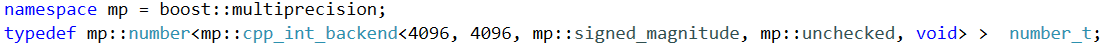
\includegraphics[width=1\textwidth]{image/number_t.PNG}
\end{center}

Như vậy ta có thể sử dụng kiểu dữ liệu mới là \textbf{number\_t} với các phép toán built-in như đối với các phép toán trên số nguyên trong C++. Điều này giúp cải thiện rất nhiều chi phí tính toán.